\documentclass{beamer}

\usetheme{default}
\usecolortheme{rose}
\usepackage{hyperref}
\newcommand{\ignore}[1]{}
\newcommand{\pr}{\mathbb{P}}
\newcommand{\E}{\mathbb{E}}
\newcommand{\var}{\text{var}}
\newcommand{\sd}{\text{sd}}
\setbeamerfont{alerted text}{series=\itshape}
\addtobeamertemplate{navigation symbols}{}{%
    \usebeamerfont{footline}%
    \usebeamercolor[fg]{footline}%
    \hspace{1em}%
    \insertframenumber/\inserttotalframenumber
}

\title{The Normal Model}

% A subtitle is optional and this may be deleted
\subtitle{STAT-UB.0001 Statistics for Business Control}

\author{Ningshan Zhang}
% - Give the names in the same order as the appear in the paper.
% - Use the \inst{?} command only if the authors have different
%   affiliation.

\institute[New York University] % (optional, but mostly needed)
{
  IOMS Department\\
  nzhang@stern.nyu.edu
  \let\thefootnote\relax\footnotetext{\tiny{*  Office Hours: Wed \& Fri 10:00 - 11:30 AM, KMC 8-174}}
}
\date{Jul 24, 2018}
\AtBeginSubsection[]
{
  \begin{frame}<beamer>{Outline}
    \tableofcontents[currentsection,currentsubsection]
  \end{frame}
}

% Let's get started
\begin{document}

%-------------------
\begin{frame}
  \titlepage
\end{frame}



% Section and subsections will appear in the presentation overview
% and table of contents.
\begin{frame}{Review: Models for Counts}
Two common distributions for counts:
\begin{itemize}
    \item Binomial distribution, $B(n,p)$
\begin{itemize}
        \item X = number of successes of $n$ independent trials, each has probability $p$ of success.
\end{itemize}
\item Poisson distribution, $\text{Poisson}(\lambda)$
\begin{itemize}
        \item X = the number of events that occur in a fixed interval, where events occur with a constant rate, and
            the events occur independently.
\end{itemize}

\end{itemize}
\end{frame}

\begin{frame}{Review: Binomial Distribution}
    \begin{figure}
        \caption{The PDF of binomial distribution $B(n,p)$.}
        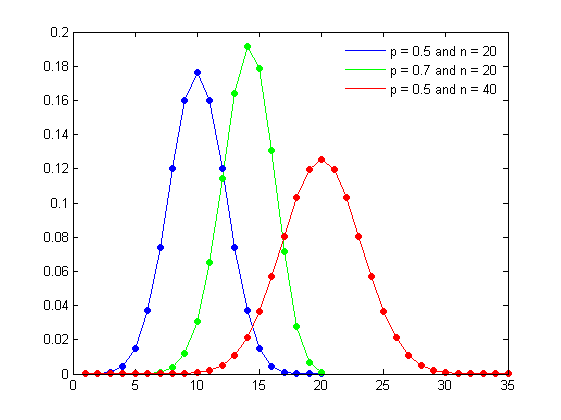
\includegraphics[width=0.8\textwidth]{figures/Binomial_distribution_pdf.png}
    \end{figure}
\end{frame}

\begin{frame}{Review: Poisson Distribution}
    When to use Poisson distribution: counting the number of successes, where
    \begin{itemize}
        \item There is a large number of trials; 
        \item The probability of success for each trial is small;
        \item The long run average number of successes within a fixed interval is known.
    \end{itemize}

    \vspace{\stretch{0.5}}
    Example: (mostly used) number of arrivals in a time window; number of emails you get in an hour; 
    number of appearances of a word in a document.
    %number of chocolate chips in a cookie.
\end{frame}

\begin{frame}{Review: Poisson Distribution}
\begin{figure}
    \caption{The PDF of Poisson distribution $\text{Poisson}(\lambda)$.}
    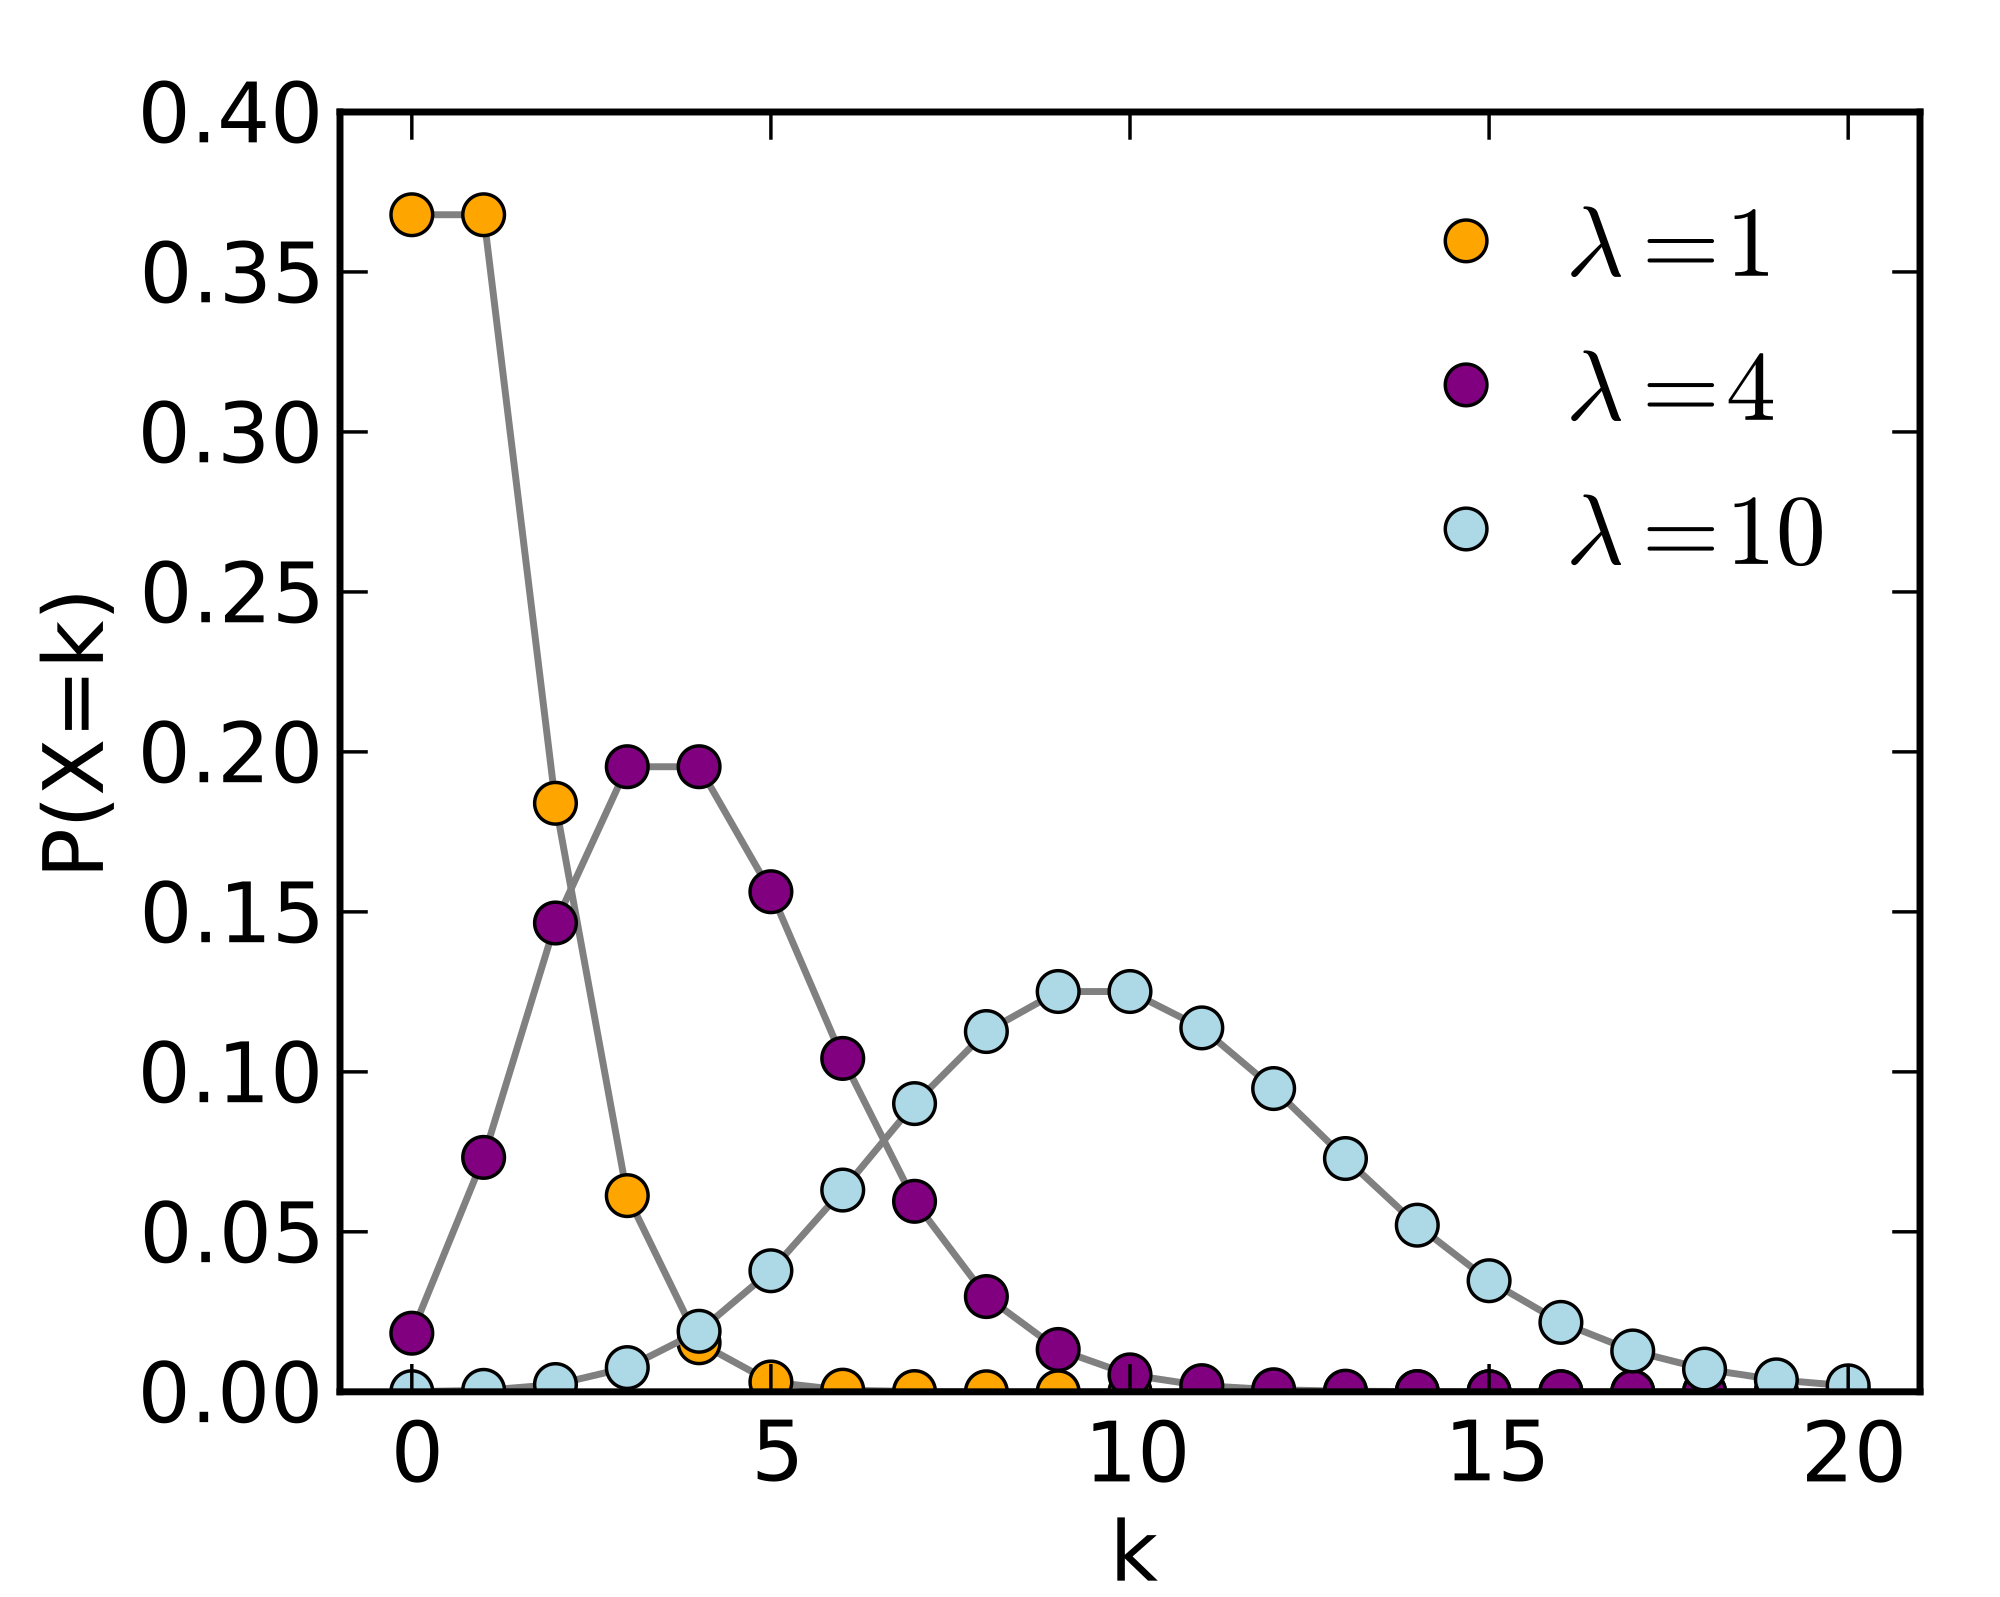
\includegraphics[width=0.8\textwidth]{figures/Poisson_pmf.png}
\end{figure}
\end{frame}

\begin{frame}{Continuous Random Variables}
Continuous random variables
\begin{itemize}
\item Can assume any value in an interval of real numbers.
\item Continuous random variables are uncountable .
\item Often ``measuring''.
\end{itemize}

\vspace{\stretch{0.5}}
Example: height, weight, etc.
\end{frame}

\begin{frame}{Continuous Random Variables: Example}
Spin a dial, let X be the angle between the dial and the horizontal (measured in degrees). 
\begin{itemize}
\vspace{\stretch{0.2}}
\item What's the probability for $X \in [0, 180]$?
\vspace{\stretch{0.2}}
\item What's the probability for $X \in [44.9, 45.1]$?
\vspace{\stretch{0.2}}
\item What's the probability for $X = 45$? 
\vspace{\stretch{0.2}}
\end{itemize}
\end{frame}

\begin{frame}{Continuous Random Variables}
X is a continuous random variable. 
\vspace{\stretch{0.1}}
\begin{itemize}
\item We do not talk about the probability of $X$ taking any \alert{individual value}:
$$\pr(X=x)=0, \text{ for any value of }x.$$
\item We talk about the probability of $X$ \alert{within a range of values}:
$$\pr(X \in [a,b]) \text{ is well defined, for any values of }a, b.$$
\end{itemize}
\end{frame}

\begin{frame}{The Probability Density Function}
The distribution of a continuous random variable is described by a smooth function, $f(x)$, 
called probability density function (pdf).
\begin{itemize}
\item Let X be a continuous random variable with pdf $f(x)$.
\item Then the probability that X is between a and b is the \alert{area under the curve} $f(x)$ between $x=a$ and $x=b$.
\end{itemize}
\begin{figure}
    \caption{The pdf and the area under the curve.}
    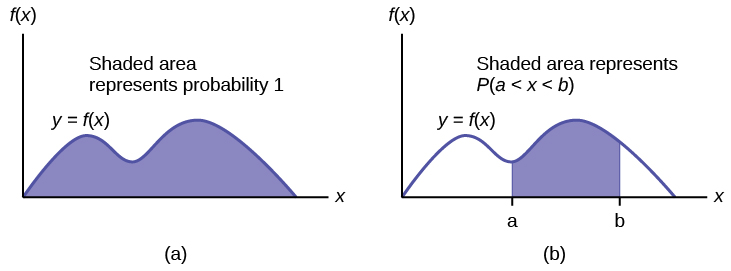
\includegraphics[width=0.8\textwidth]{figures/pdf.jpg}
\end{figure}
\end{frame}

\begin{frame}{The Probability Density Function}
\begin{itemize}
\item Using calculus, the probability that $X$ is between $a$ and $b$ is computed as
$$
\pr(a < X < b) = \int_{a}^b f(x)dx.
$$

\item Properties of the probability density function $f(x)$:
$$ f(x)\geq 0, \quad \int_{-\infty}^{\infty} f(x)dx=1.$$
\end{itemize}


\let\thefootnote\relax\footnotetext{\tiny{* Note: In this class, you will not need to evaluate any integrals.}}
\end{frame}

\begin{frame}{Expected Value and Variance}
Let X be a continuous random variable with pdf $f(x)$.
\vspace{\stretch{0.1}}
\begin{itemize}
\item The expected value (or mean) of $X$ is
$$ \E (X) = \mu = \int_{-\infty}^{\infty} x f(x) dx.$$
\item The variance of $X$ is
$$ \var (X) = \sigma^2 = \int_{-\infty}^{\infty} (x-\mu)^2 f(x) dx.$$
\end{itemize}

\let\thefootnote\relax\footnotetext{\tiny{* Note: In this class, we will not compute these directly via integrals.  }}
\end{frame}


\begin{frame}{The Normal Distribution}
\begin{figure}
    \caption{The pdf of a normal distribution with mean $\mu$ and variance $\sigma^2$.}
    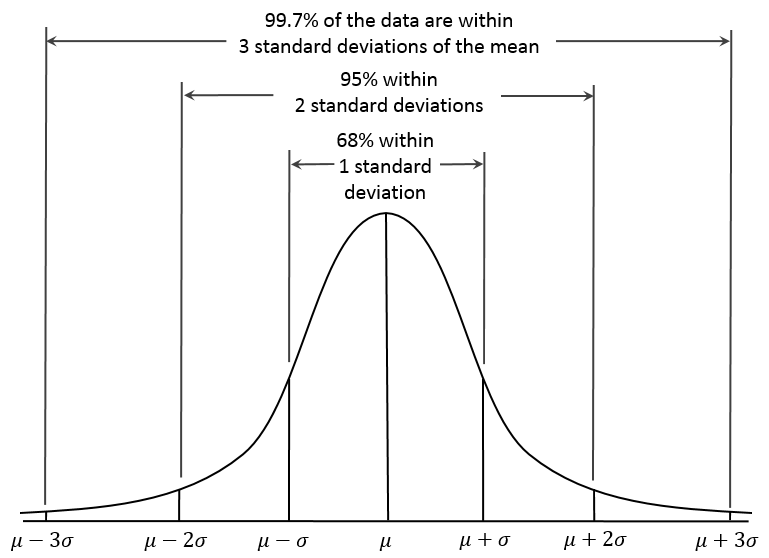
\includegraphics[width=0.8\textwidth]{figures/normal_pdf.png}
\end{figure}
\end{frame}

\begin{frame}{The Normal Distribution}
The normal distribution is the most important distribution for a continuous random variable.  Why is it so important?
\begin{itemize}
\item It’s mathematically ``convenient''.
\item Many things in the world are approximately normally distributed. If not, can be transformed into normal, e.g. take log.
\item (Most important) Sample means tend to have normal distributions, even if the distribution of the population that we’re sampling from does not (more on this later).
\end{itemize}
\end{frame}


\begin{frame}{The Normal Distribution}
The pdf for the normal distribution with mean $\mu$ and variance $\sigma^2$ is:
$$
f(x) = \frac{1}{\sigma\sqrt{2\pi} } e^{-\frac{(x-\mu)^2}{2\sigma^2}}.
$$

\begin{itemize}
\item It is a bell-shaped, continuous function.
\item It has two parameters: $\mu$ (mean) and $\sigma$ (standard deviation).
\item It is symmetrical about $\mu$ and its maximum is at $\mu$.
\end{itemize}

\vspace{\stretch{0.2}}
If $X$ is a normal random variable with mean $\mu$ and variance $\sigma^2$, we usually write $ X \sim \mathcal{N}(\mu,\sigma^2)$.
\let\thefootnote\relax\footnotetext{\tiny{* Note: In this class, we will not work directly with this pdf.  }}
\end{frame}

\ignore{
\begin{frame}{The Normal Distribution}
Characteristics of the pdf of a normal distribution:
\begin{itemize}
\item It is a bell-shaped, continuous function.
\item It has two parameters: $\mu$ (mean) and $\sigma^2$ (variance).
\item It is symmetrical about $\mu$ and its maximum is at $\mu$.
\item The inflection points of $f(x)$ are at $\mu-\sigma$ and $\mu+\sigma$.
\end{itemize}

\vspace{\stretch{0.5}}
Notation: a normal distribution with mean $\mu$ and variance $\sigma^2$ is written as $\mathcal{N}(\mu,\sigma^2)$.
\end{frame}
}


\begin{frame}{ The \alert{Standard} Normal Distribution}
Standard normal distribution:
\begin{itemize}
\item A normal distribution with $\mu=0$ and $\sigma=1$. The simplest normal distribution.
\item Denote a standard normal random variable by $Z$.
\item No analytical solution for $\pr(a<Z<b)$ for arbitrary $a,b$. 
\item People use a precomputed table to find the areas under the curve for $Z$.
\end{itemize}
\end{frame}

\begin{frame}{The Cumulative Distribution Function}
    The cumulative distribution function (CDF) of random variable $X$ is defined as
    $$ F(x) = \pr(X\leq x ).$$
    \begin{itemize}
    \item The CDF of the standard normal distribution is usually denoted by $\Phi(x)$.
    \end{itemize}
\begin{figure}
    \caption{The $\Phi$ function (CDF of standard normal $Z$).}
    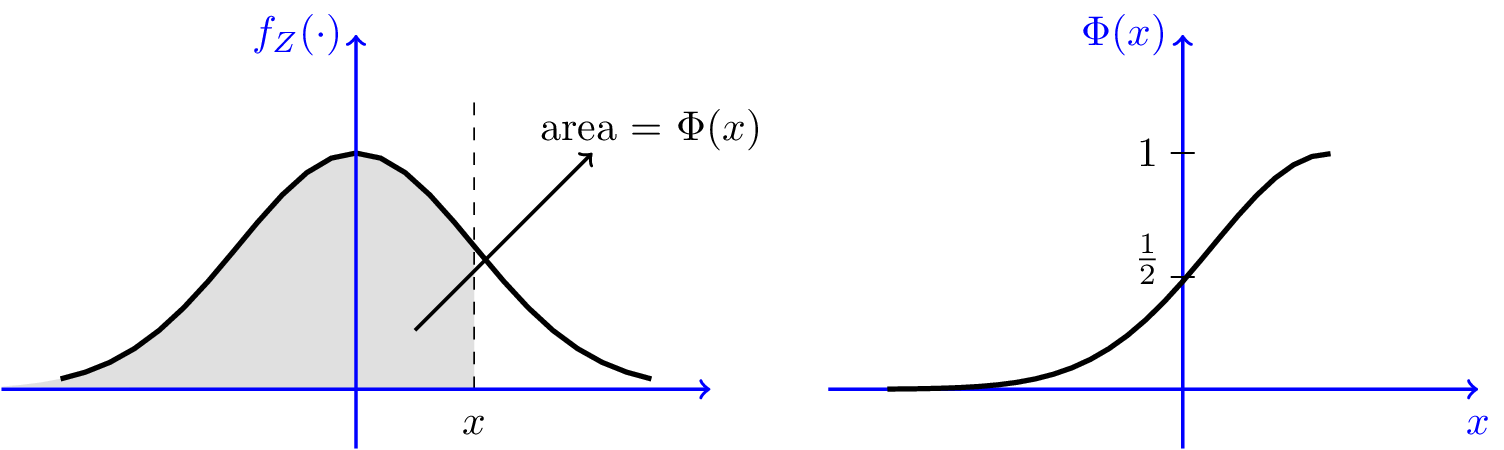
\includegraphics[width=0.8\textwidth]{figures/phi.png}
\end{figure}
\end{frame}

\begin{frame}{Z-table: the Normal CDF Table}
    Suppose $Z$ is a standard normal random variable. What is $\pr (Z \leq 1.2)$?

\vspace{\stretch{0.5}}
\begin{figure}
    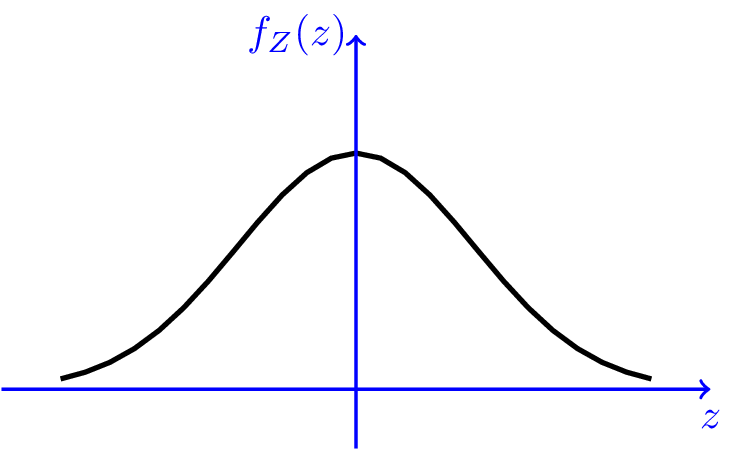
\includegraphics[width=0.5\textwidth]{figures/empty_pdf.png}
\end{figure}
\end{frame}

\begin{frame}{Z-table: the Normal CDF Table}
    Suppose $Z$ is a standard normal random variable. What is $\pr (Z \leq -0.4)$?

\vspace{\stretch{0.5}}
\begin{figure}
    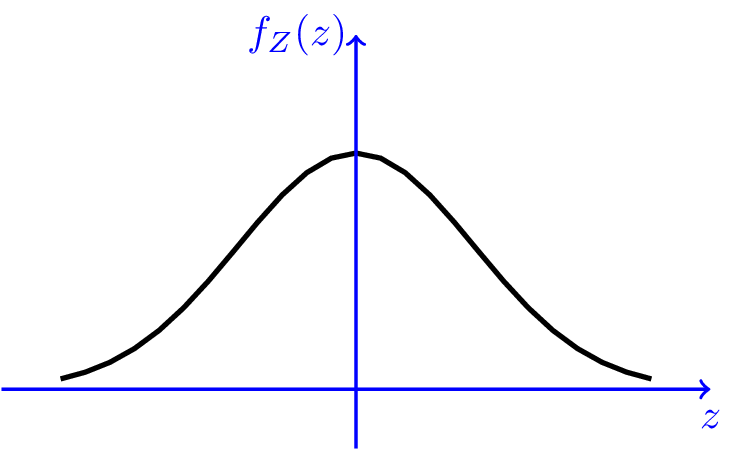
\includegraphics[width=0.5\textwidth]{figures/empty_pdf.png}
\end{figure}
\end{frame}

\begin{frame}{Z-table: the Normal CDF Table}
    Suppose $Z$ is a standard normal random variable. What is $\pr (-0.4 < Z \leq 1.2)$?

\vspace{\stretch{0.5}}
\begin{figure}
    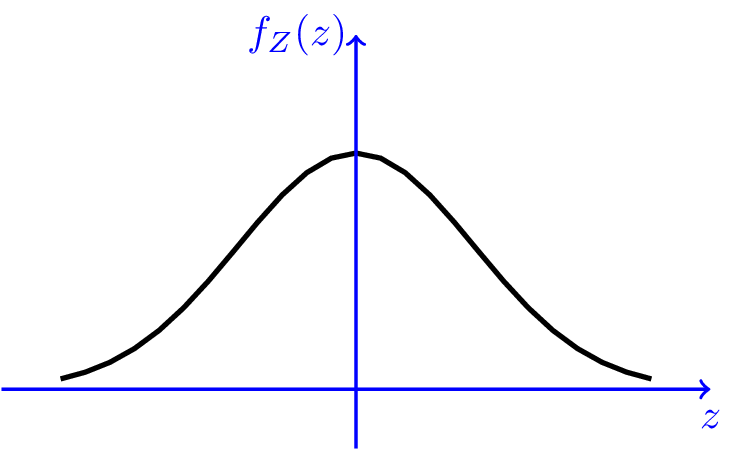
\includegraphics[width=0.5\textwidth]{figures/empty_pdf.png}
\end{figure}
\end{frame}

\begin{frame}{Z-table: the Inverse Normal CDF Table}
    Suppose $Z$ is a standard normal random variable. 
    Find $z$ such that $\pr(Z \leq z) =0.60$.

\vspace{\stretch{0.5}}
\begin{figure}
    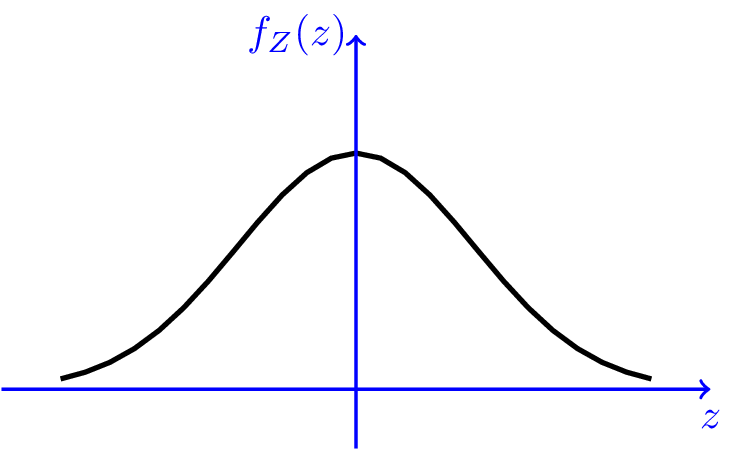
\includegraphics[width=0.5\textwidth]{figures/empty_pdf.png}
\end{figure}
\end{frame}

\begin{frame}{Z-table: the Inverse Normal CDF Table}
    Suppose $Z$ is a standard normal random variable. 
    Find $z$ such that $\pr(-z \leq Z \leq z) =0.95$.


\vspace{\stretch{0.5}}
\begin{figure}
    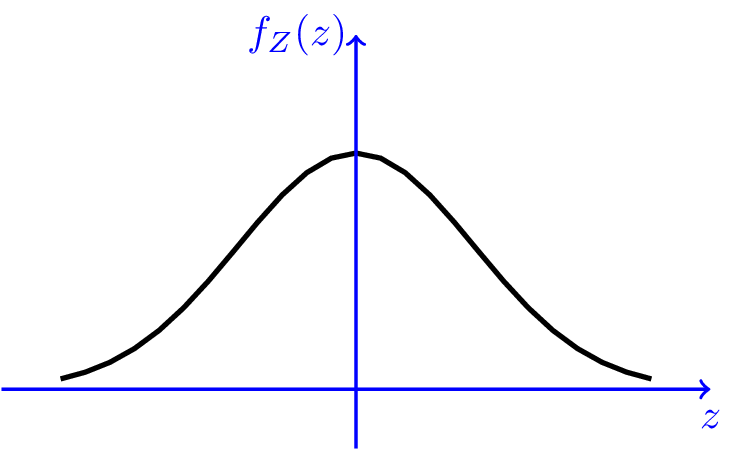
\includegraphics[width=0.5\textwidth]{figures/empty_pdf.png}
\end{figure}
\end{frame}

\begin{frame}{Z-tables}
    Two tables contain the same information. 
    \vspace{\stretch{0.1}}
    \begin{itemize}
        \item Normal CDF Table: the cutoff \alert{$z$ values} are rounded. It is used to look up for probabilities.
        \item Inverse Normal CDF Table: the \alert{probabilities} are rounded. It is used to look up for cutoff $z$ values.
    \end{itemize}
\end{frame}

\begin{frame}{Convert Normal to Standard Normal}
    Shifting and rescaling property.
    \begin{itemize}
        \item If $X$ is a \alert{normal} with mean $\mu$ and standard deviation $\sigma$, and $a,b$ are two constants. 
            Then, 
            %$$ aX+b \sim \mathcal{N}(a\mu+b,a^2\sigma^2).$$
            $aX+b$ is a \alert{normal} with mean $a\mu+b$ and standard deviation $|a|\sigma$.
            $$ X \sim \mathcal{N}(\mu,\sigma^2) \Rightarrow aX+b \sim \mathcal{N}(a\mu+b,a^2\sigma^2).$$
        \item In particular, $Z=\frac{X-\mu}{\sigma}$ is a standard normal:
            \begin{align*}
                \E\big(\frac{X-\mu}{\sigma}\big) &= \frac{\mu-\mu}{\sigma}=0,\\
                \sd\big(\frac{X-\mu}{\sigma}\big) &= \frac{\sigma}{\sigma} =1.
            \end{align*}
    \end{itemize}
\end{frame}


\begin{frame}{Summary}
Continuous random variables
\begin{itemize}
\item Probability density function (pdf)
\item Area under the curve
\end{itemize}
\vspace{\stretch{0.2}}
Normal distribution
\begin{itemize}
\item Normal distribution's pdf
\item Standard normal distribution, z-tables
\item Convert normal to standard normal
\end{itemize}
\end{frame}

\ignore{
%-------------------
\begin{frame}{Time Series Plot}
\begin{figure}
    \caption{}
    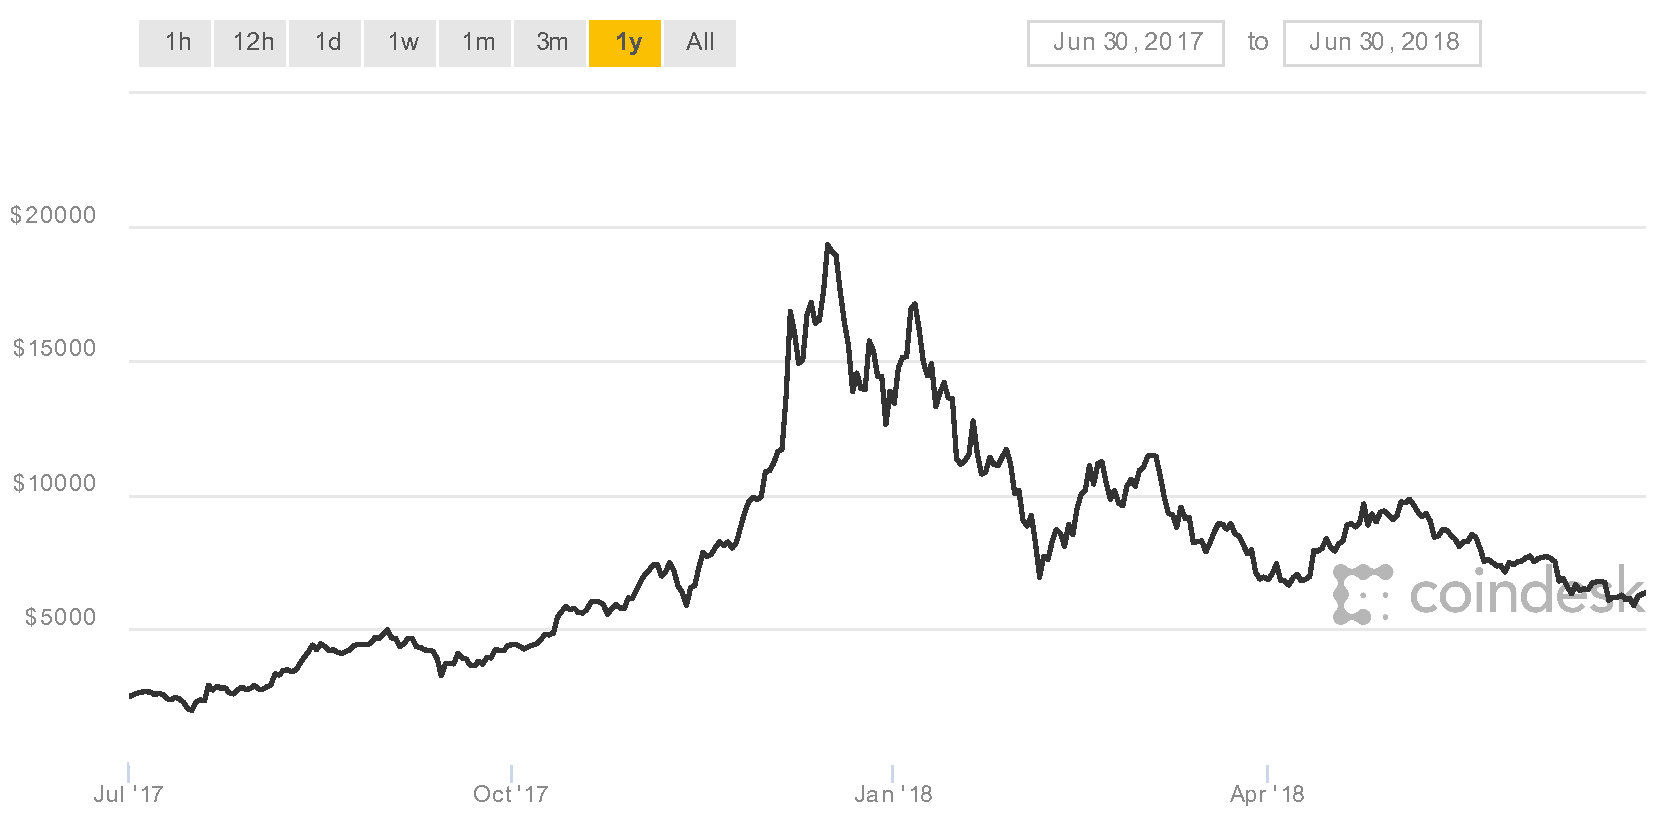
\includegraphics[width=1\textwidth]{figures/coindesk-bpi-chart}
\end{figure}
\let\thefootnote\relax\footnotetext{\tiny{* Plot from Coindesk.com}}
\end{frame}

\begin{frame}{}
\begin{itemize}
\item 
\end{itemize}
\end{frame}

\vspace{\stretch{0.5}}

\begin{block}{}
\end{block}


}

\end{document}


